\documentclass[conference]{IEEEtran}
\IEEEoverridecommandlockouts
\usepackage{cite}
\usepackage{amsmath,amssymb,amsfonts}
\usepackage{graphicx}
\usepackage{textcomp}
\usepackage{booktabs}
\usepackage{multirow}
\usepackage{xcolor}
\usepackage{tikz}
\usetikzlibrary{positioning,arrows.meta}
\usepackage{url}
\def\BibTeX{{\rm B\kern-.05em{\sc i\kern-.025em b}\kern-.08em
    T\kern-.1667em\lower.7ex\hbox{\sc e}\kern-.125em\scalebox{0.85}{X}}}

\begin{document}

\title{When 99\% Is Not Evidence: Benchmark Leakage, Model Comparison and Explanation Disagreement in Crop and Fertilizer Recommendation}

% TODO: replace with the real author names, departments and e-mails.
\author{\IEEEauthorblockN{Author One}
\IEEEauthorblockA{\textit{Dept. of Computer Science and Engineering} \\
\textit{University Name}\\
City, India \\
author1@example.com}
\and
\IEEEauthorblockN{Author Two}
\IEEEauthorblockA{\textit{Dept. of Computer Science and Engineering} \\
\textit{University Name}\\
City, India \\
author2@example.com}
\and
\IEEEauthorblockN{Guide Name}
\IEEEauthorblockA{\textit{Dept. of Computer Science and Engineering} \\
\textit{University Name}\\
City, India \\
guide@example.com}
}

\maketitle

\begin{abstract}
Machine learning papers on crop recommendation routinely report accuracies above 95\% on the public Kaggle crop dataset, and fertilizer papers report near-perfect accuracy on a 99-row ``Fertilizer Prediction'' dataset. We test what these numbers measure. We compare 16 classifiers on the crop dataset with 5$\times$5 repeated stratified cross-validation and a corrected resampled $t$-test, diagnose overfitting with train/test gaps, complexity curves and a label-permutation test, and trace the dataset to its creator's notebook. The best model (Stacking) reaches 99.57\% accuracy, but 11 of 16 models are not significantly worse, including Gaussian Naive Bayes (99.47\%) and a single decision tree (98.80\%). The models are not overfitting: train/test gaps are 0.06 to 2.5 percentage points. Instead, the N, P and K columns were generated from the label: all 2,200 rows satisfy the creator's rule $N=\text{base}_N[\text{crop}]+U\{-20,20\}$, and a lookup of the 22-row base table identifies the crop from N, P, K with 65.8\% expected accuracy and no learning. On the fertilizer dataset, N, P and K alone give 100\% leave-one-out accuracy, while temperature, humidity and moisture give 16--25\% and soil plus crop type 9--17\%, below the 22\% majority class; each class's median N:P:K is closest to the grade of the fertilizer in its own label. SHAP and LIME agree on the top feature in 80\% of instances, and both attribute 23--36\% of the fertilizer model to features that carry no information. We conclude that these benchmarks measure recovery of a generating rule, not agronomic skill, and we describe the evaluation a real-data study needs.
\end{abstract}

\begin{IEEEkeywords}
Crop recommendation, fertilizer recommendation, benchmark leakage, model comparison, explainable AI, SHAP, LIME, conformal prediction
\end{IEEEkeywords}

\section{Introduction}

Choosing which crop to grow and how much fertilizer to apply are the two decisions a farmer makes every season, and both have attracted a large body of machine learning work. Most of this work follows one template: take the public Kaggle ``Crop Recommendation'' dataset \cite{kaggle_crop}, with seven features (N, P, K, temperature, humidity, pH, rainfall) and 22 crops, train several classifiers, and report the one with the highest accuracy, usually above 95\%. Fertilizer recommendation follows the same template on a 99-row dataset that maps soil and weather readings to one of seven fertilizer names.

A model that scores 99\% looks ready to advise farmers. Before accepting that, three questions need answers. Is the difference between the best model and the rest real, or within the noise of the split? Is the high score a sign of overfitting, or of something in the data? And when an explanation method such as SHAP \cite{lundberg2017} says which feature drove a recommendation, does a second method agree, and does the explanation point to something a farmer could change?

We answer these questions with experiments, not argument. Our main contributions are:
\begin{itemize}
\item A comparison of 16 classifiers on the crop dataset under 5$\times$5 repeated stratified cross-validation with a corrected resampled $t$-test \cite{nadeau2003,bouckaert2004} and Holm adjustment \cite{holm1979}: 11 of the other 15 models are statistically tied with the best.
\item A diagnosis that separates overfitting from leakage \cite{kaufman2012,kapoor2023}: train/test gaps, complexity curves and a label-permutation test \cite{ojala2010} rule out overfitting, and the creator's notebook \cite{harvestify} shows that N, P, K were generated from the label. We verify this for 2,200 of 2,200 rows.
\item A comparison of feature groups and models on the fertilizer dataset showing that the N:P:K inputs mirror the nutrient grade of the fertilizer named in the label, and a soil-test alternative that converts a nutrient dose into product quantities.
\item An evaluation of the explanations themselves: SHAP versus LIME \cite{ribeiro2016} agreement, a deletion test, a pure-noise feature check and constrained counterfactuals \cite{wachter2018,ustun2019}, plus calibration \cite{guo2017} and conformal prediction sets \cite{sadinle2019,romano2020}.
\end{itemize}

The paper is organised as follows. Section~II gives background and related work. Section~III describes the datasets and the evaluation protocol. Section~IV presents the results for crop and fertilizer recommendation and discusses them. Section~V concludes and lists the real-data work that follows.

\section{Background}

\subsection{Preliminary Concepts}

\subsubsection{Models compared}
We compare 16 classifiers that cover the families used in the crop recommendation literature (Table~\ref{tab:models}): linear (logistic regression), probabilistic (Gaussian Naive Bayes), instance-based ($k$-NN), kernel (RBF-SVM), a single decision tree, bagged trees (Random Forest \cite{breiman2001}, Extra Trees, Bagging), boosted trees (AdaBoost \cite{freund1997,zhu2009}, histogram gradient boosting, XGBoost \cite{chen2016}, LightGBM \cite{ke2017}, CatBoost \cite{prokhorenkova2018}), a multilayer perceptron, and two ensembles (soft voting and stacking \cite{wolpert1992}). All models use scikit-learn \cite{pedregosa2011} or the libraries' own implementations.

\begin{table}[htbp]
\caption{Models Compared and Their Fixed Settings (Not Tuned)}
\label{tab:models}
\centering
\footnotesize
\begin{tabular}{@{}ll@{}}
\toprule
\textbf{Model} & \textbf{Setting} \\
\midrule
Logistic Regression & standardised, $C=10$ \\
Gaussian NB & default \\
KNN & standardised, $k=5$, distance wts. \\
SVM (RBF) & standardised, $C=10$, $\gamma$=scale \\
Decision Tree & unpruned \\
Random Forest / Extra Trees & 300 trees \\
Bagging & 100 unpruned trees \\
AdaBoost & depth-3 trees, 200 rounds, lr 0.5 \\
HGB, XGBoost, LightGBM, CatBoost & defaults \\
MLP & 128--64 units, early stopping \\
Soft Voting & RF + XGBoost + LightGBM \\
Stacking & RF, ET, SVM, LightGBM $\rightarrow$ LR \\
\bottomrule
\end{tabular}
\end{table}

Hyperparameters are fixed in advance and not tuned on the data; the same settings are used in every experiment. With the scores reported below, tuning cannot separate the models in any meaningful way.

\subsubsection{SHapley Additive exPlanations (SHAP)}
SHAP \cite{lundberg2017} decomposes a model's output for input $\mathbf{x}$ into per-feature contributions,
\begin{equation}
f(\mathbf{x}) = \phi_0 + \sum_{j=1}^{M}\phi_j ,
\end{equation}
where $\phi_0$ is the expected output and $\phi_j$ is the Shapley value of feature $j$. For tree ensembles TreeSHAP computes these values exactly in polynomial time \cite{lundberg2020}.

\subsubsection{LIME}
LIME \cite{ribeiro2016} fits a sparse linear model to the classifier's outputs on perturbed copies of one instance and reports its coefficients as the explanation. SHAP and LIME answer slightly different questions, so they can disagree \cite{krishna2024}.

\subsubsection{Conformal prediction}
Split conformal prediction returns a set of crops $C(\mathbf{x})$ that contains the true crop with probability at least $1-\alpha$. With the least ambiguous set-valued classifier (LAC) \cite{sadinle2019}, the score is $s(\mathbf{x},y)=1-\hat p_y(\mathbf{x})$ and
\begin{equation}
C(\mathbf{x}) = \{\,y : 1-\hat p_y(\mathbf{x}) \le \hat q\,\},
\end{equation}
where $\hat q$ is the $\lceil (n+1)(1-\alpha)\rceil/n$ quantile of the scores on $n$ calibration rows. Adaptive prediction sets (APS) \cite{romano2020} accumulate sorted probabilities instead. See \cite{angelopoulos2021} for an introduction.

\subsection{Related Work}

\textit{Crop and fertilizer recommendation.} The Kaggle crop dataset \cite{kaggle_crop} is the most common benchmark for crop recommendation. Its creator's repository, Harvestify \cite{harvestify}, describes it as a ``custom built dataset'' and warns not to use it for farming decisions. The fertilizer dataset is used the same way, as a 7-class classification task.

\textit{Leakage.} Leakage occurs when the features contain information about the label that would not be available at prediction time \cite{kaufman2012}. Kapoor and Narayanan found leakage behind reproducibility failures in many ML-based studies across 17 fields \cite{kapoor2023}. A dataset whose features were generated from its label is an extreme case.

\textit{Model comparison.} Comparing classifiers by mean accuracy on repeated splits overstates significance because the training sets overlap; the corrected resampled $t$-test accounts for this \cite{nadeau2003,bouckaert2004}. On tabular data, tree ensembles remain strong baselines against deep models \cite{grinsztajn2022}.

\textit{Spatial validation.} When observations are spatially correlated, random cross-validation overestimates accuracy and block or leave-region-out validation is needed \cite{roberts2017}. The crop benchmark has no location field, so this cannot be tested on it.

\textit{Evaluating explanations.} Explanation methods disagree with each other \cite{krishna2024}. Counterfactual explanations state the smallest change that alters a prediction \cite{wachter2018}, and actionable recourse restricts that change to features a person can control \cite{ustun2019}.

That is the gap we address: published crop and fertilizer results are reported without significance tests, without checking where the data came from, and without testing the explanations they show.

\section{Proposed Approach}

\subsection{Datasets}

\textit{Crop dataset.} 2,200 rows, 22 crops with exactly 100 rows each, seven features, no missing values and no duplicate rows \cite{kaggle_crop}. The creator's notebook \cite{harvestify} builds each row from a 22-row table of base values per crop:
\begin{equation}
\begin{aligned}
N &= \text{base}_N[c] + U\{-20,20\},\\
P &= \text{base}_P[c] + U\{-5,20\},\\
K &= \text{base}_K[c] + U\{-5,5\},
\end{aligned}
\label{eq:gen}
\end{equation}
where $c$ is the crop label and $U\{a,b\}$ is a uniform random integer. Temperature, humidity, pH and rainfall are copied from a second file whose origin is not documented.

\textit{Fertilizer dataset.} 99 rows, seven fertilizer classes (Urea 22, DAP 18, 28-28 17, 14-35-14 14, 20-20 14, 17-17-17 7, 10-26-26 7) and eight inputs: temperature, humidity, moisture, soil type, crop type, N, P and K. Its construction is not documented.

\subsection{Evaluation Protocol}

\subsubsection{Model comparison}
Each model is trained and tested on the same 25 splits (5-fold stratified cross-validation repeated 5 times). We report accuracy, macro-F1, top-3 accuracy, log-loss, expected calibration error (ECE, 15 bins) and fit time. Each model is compared with the best by the corrected resampled $t$-statistic
\begin{equation}
t = \frac{\bar d}{\sqrt{\left(\frac{1}{kr} + \frac{n_2}{n_1}\right)\hat\sigma_d^2}},
\end{equation}
where $\bar d$ and $\hat\sigma_d^2$ are the mean and variance of the macro-F1 differences over the $kr=25$ splits and $n_2/n_1$ is the test-to-train size ratio \cite{nadeau2003}. $p$-values are Holm-adjusted for 15 comparisons.

\subsubsection{Overfitting versus leakage}
Overfitting shows as a gap between training and held-out accuracy. We measure that gap for 11 models, plot accuracy against decision-tree depth and $k$ in $k$-NN, and run a label-permutation test with 100 permutations \cite{ojala2010}. We then check every row against (\ref{eq:gen}) and compute the accuracy of a zero-learning lookup: for each row, the crops whose generator box contains its (N, P, K), with ties split uniformly.

\subsubsection{Robustness}
Learning curves use 2 to 80 training rows per crop. Measurement noise adds Gaussian noise with standard deviation $k$ times each feature's standard deviation to the test rows. Feature ablation removes one feature at a time and compares soil-only (N, P, K, pH) with climate-only features.

\subsubsection{Explanations}
For 200 test instances we compare SHAP and LIME (2,000 perturbations) by top-3 overlap, same top feature, Spearman correlation and sign agreement. In the deletion test we set the top-$k$ features to their median and record the predicted crop's probability; a faithful ranking should drop it faster than a random one. We add one pure-noise feature and record the share of attribution it receives. Stability across splits is measured with Kendall's $W$. Counterfactuals keep climate fixed and change only N, P, K and pH.

\subsubsection{Fertilizer}
On the fertilizer data we use leave-one-out accuracy for four models and four feature groups, against the majority class. For each class we take the median (N, P, K) and compute its cosine similarity with the N--P$_2$O$_5$--K$_2$O grade $\mathbf{g}$ of every product:
\begin{equation}
\cos(\mathbf{m}_c,\mathbf{g}) = \frac{\mathbf{m}_c\cdot\mathbf{g}}{\lVert\mathbf{m}_c\rVert\,\lVert\mathbf{g}\rVert}.
\end{equation}
If the inputs mirror the label, each class is most similar to its own product. Finally we convert a nutrient dose into product quantities: P$_2$O$_5$ comes only from DAP (18-46-0), the remaining N from urea (46-0-0) and K$_2$O from MOP (0-0-60):
\begin{equation}
\text{DAP} = \frac{P_2O_5}{0.46},\quad
\text{Urea} = \frac{N - 0.18\,\text{DAP}}{0.46},\quad
\text{MOP} = \frac{K_2O}{0.60}.
\label{eq:dose}
\end{equation}

\subsection{Experimental Pipeline}

The pipeline is shown in Fig.~\ref{fig:pipeline}. All experiments use seed 42 and run on CPU.

\begin{figure}[htbp]
\centering
\footnotesize
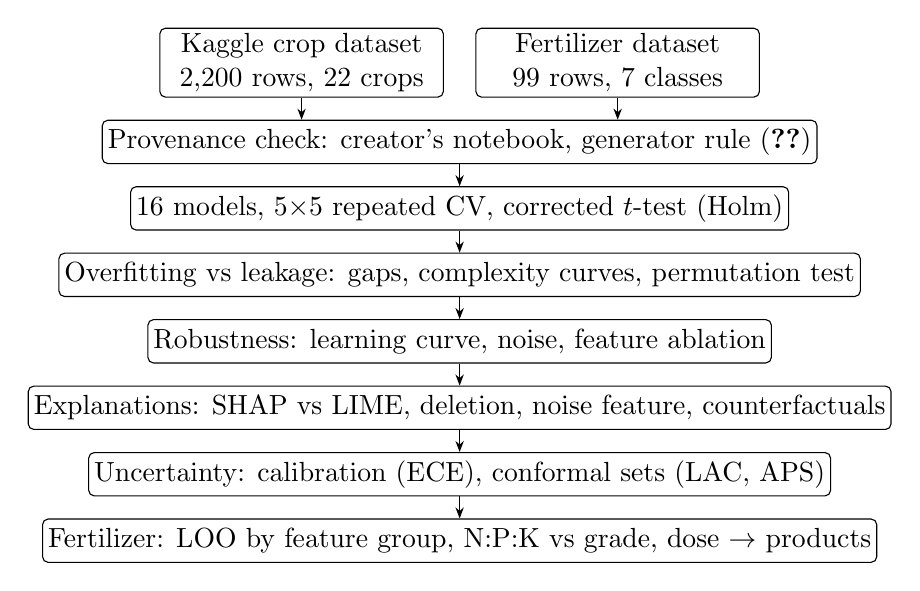
\begin{tikzpicture}[
  box/.style={draw, rounded corners=2pt, align=center, minimum width=7.6cm, minimum height=0.55cm, inner sep=2pt},
  sbox/.style={draw, rounded corners=2pt, align=center, minimum width=3.6cm, minimum height=0.55cm, inner sep=2pt},
  arr/.style={-{Stealth[length=4pt]}}, node distance=0.28cm]
\node[sbox] (k) {Kaggle crop dataset\\2,200 rows, 22 crops};
\node[sbox, right=0.4cm of k] (f) {Fertilizer dataset\\99 rows, 7 classes};
\node[box, below=of k.south east, anchor=north, xshift=0.2cm] (p) {Provenance check: creator's notebook, generator rule (\ref{eq:gen})};
\node[box, below=of p] (m) {16 models, 5$\times$5 repeated CV, corrected $t$-test (Holm)};
\node[box, below=of m] (o) {Overfitting vs leakage: gaps, complexity curves, permutation test};
\node[box, below=of o] (r) {Robustness: learning curve, noise, feature ablation};
\node[box, below=of r] (x) {Explanations: SHAP vs LIME, deletion, noise feature, counterfactuals};
\node[box, below=of x] (u) {Uncertainty: calibration (ECE), conformal sets (LAC, APS)};
\node[box, below=of u] (fz) {Fertilizer: LOO by feature group, N:P:K vs grade, dose $\rightarrow$ products};
\draw[arr] (k) -- (k |- p.north);
\draw[arr] (f.south) -- (f |- p.north);
\draw[arr] (p) -- (m); \draw[arr] (m) -- (o); \draw[arr] (o) -- (r);
\draw[arr] (r) -- (x); \draw[arr] (x) -- (u); \draw[arr] (u) -- (fz);
\end{tikzpicture}
\caption{Experimental pipeline. Both public benchmarks go through a provenance check, then the same evaluation stages; the fertilizer dataset also gets a grade-matching test and a dose-to-product conversion.}
\label{fig:pipeline}
\end{figure}

\section{Results and Discussion}

\subsection{Experimental Setup}

Experiments use Python with scikit-learn \cite{pedregosa2011}, XGBoost, LightGBM, CatBoost, SHAP and LIME, and run on a CPU. Every number below is read from a result file produced by the experiment scripts; the ledger \texttt{results/CLAIMS.md} maps each number to its file.

\subsection{Comparison of Machine Learning Models}

Table~\ref{tab:bench} and Fig.~\ref{fig:bench} give the comparison. Stacking has the highest mean accuracy, 99.57\%. Eleven of the other 15 models, from soft voting (99.54\%) down to the single decision tree (98.80\%), are not significantly worse after Holm adjustment. Only SVM, logistic regression, $k$-NN and the MLP are significantly worse, and the worst of them, the MLP, still reaches 96.18\%.

\begin{table*}[htbp]
\caption{Model Comparison on the Kaggle Crop Dataset (Mean $\pm$ Standard Deviation Over 25 Splits of 5$\times$5 Repeated Stratified CV). Holm $p$: Corrected Resampled $t$-Test Against the Best Model on Macro-F1}
\label{tab:bench}
\centering
\footnotesize
\begin{tabular}{@{}lccccccc@{}}
\toprule
\textbf{Model} & \textbf{Accuracy (\%)} & \textbf{Macro-F1 (\%)} & \textbf{Top-3 (\%)} & \textbf{Log-loss} & \textbf{ECE} & \textbf{Fit time (s)} & \textbf{Holm $p$} \\
\midrule
Stacking (RF, ET, SVM, LGBM $\rightarrow$ LR) & 99.57 $\pm$ 0.26 & 99.57 $\pm$ 0.26 & 100.0 $\pm$ 0.0 & 0.035 & 0.027 & 14.13 & -- \\
Soft Voting (RF + XGB + LGBM) & 99.54 $\pm$ 0.25 & 99.53 $\pm$ 0.25 & 100.0 $\pm$ 0.0 & 0.031 & 0.022 & 17.86 & 1.000 \\
Random Forest & 99.52 $\pm$ 0.28 & 99.52 $\pm$ 0.28 & 100.0 $\pm$ 0.0 & 0.052 & 0.041 & 0.61 & 1.000 \\
Gaussian NB & 99.47 $\pm$ 0.24 & 99.47 $\pm$ 0.24 & 100.0 $\pm$ 0.0 & 0.015 & 0.007 & 0.00 & 1.000 \\
CatBoost & 99.36 $\pm$ 0.43 & 99.36 $\pm$ 0.43 & 100.0 $\pm$ 0.0 & 0.022 & 0.013 & 4.72 & 1.000 \\
Extra Trees & 99.32 $\pm$ 0.31 & 99.32 $\pm$ 0.31 & 100.0 $\pm$ 0.0 & 0.097 & 0.078 & 0.45 & 1.000 \\
XGBoost & 99.29 $\pm$ 0.40 & 99.29 $\pm$ 0.40 & 99.93 $\pm$ 0.17 & 0.030 & 0.013 & 0.87 & 1.000 \\
Bagging (DT) & 99.21 $\pm$ 0.42 & 99.21 $\pm$ 0.42 & 100.0 $\pm$ 0.0 & 0.028 & 0.013 & 0.34 & 1.000 \\
AdaBoost (tree d=3) & 99.19 $\pm$ 0.43 & 99.19 $\pm$ 0.43 & 99.96 $\pm$ 0.11 & 3.079 & 0.946 & 0.80 & 0.530 \\
Hist.\ Gradient Boosting & 99.06 $\pm$ 0.44 & 99.06 $\pm$ 0.44 & 99.91 $\pm$ 0.21 & 0.041 & 0.008 & 1.80 & 0.485 \\
LightGBM & 99.03 $\pm$ 0.46 & 99.02 $\pm$ 0.46 & 99.92 $\pm$ 0.21 & 0.038 & 0.008 & 1.52 & 0.441 \\
SVM (RBF) & 98.85 $\pm$ 0.29 & 98.84 $\pm$ 0.30 & 100.0 $\pm$ 0.0 & 0.143 & 0.111 & 0.12 & \textbf{0.003} \\
Decision Tree & 98.80 $\pm$ 0.69 & 98.80 $\pm$ 0.69 & 99.05 $\pm$ 0.66 & 0.414 & 0.012 & 0.01 & 0.530 \\
Logistic Regression & 97.92 $\pm$ 0.49 & 97.91 $\pm$ 0.49 & 100.0 $\pm$ 0.0 & 0.082 & 0.039 & 0.06 & \textbf{0.000} \\
KNN ($k$=5) & 97.60 $\pm$ 0.61 & 97.59 $\pm$ 0.61 & 99.69 $\pm$ 0.22 & 0.190 & 0.020 & 0.00 & \textbf{0.000} \\
MLP (128-64) & 96.18 $\pm$ 0.88 & 96.17 $\pm$ 0.88 & 99.93 $\pm$ 0.14 & 0.167 & 0.081 & 0.72 & \textbf{0.000} \\
\bottomrule
\end{tabular}
\end{table*}

\begin{figure}[htbp]
\centerline{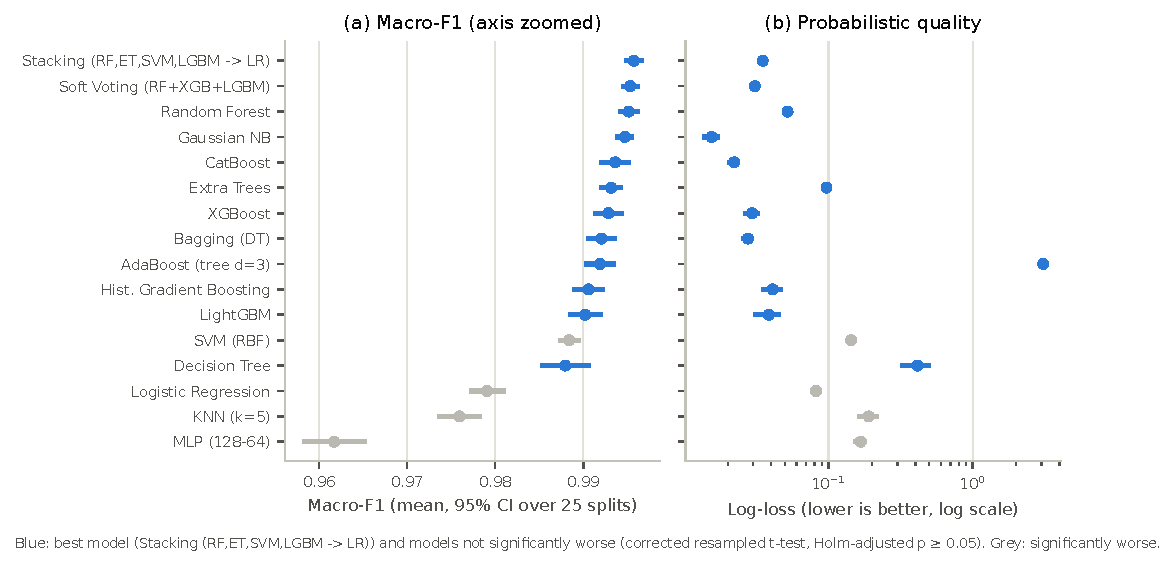
\includegraphics[width=\columnwidth]{figures/fig04_model_comparison.pdf}}
\caption{Model comparison. (a) Macro-F1 with 95\% intervals over 25 splits, axis zoomed. Blue: the best model and models not significantly worse; grey: significantly worse. (b) Log-loss on a log scale.}
\label{fig:bench}
\end{figure}

The ranking therefore says little. Gaussian Naive Bayes fits in under 0.01~s and ties with a 14-second stacked ensemble; it also has the lowest log-loss (0.015) and ECE (0.007). AdaBoost with depth-3 trees ties on accuracy but has a log-loss of 3.079 and an ECE of 0.946, because its scores are not probabilities.

\textit{The AdaBoost anomaly.} With its default weak learner, AdaBoost scores far below every other model. Fig.~\ref{fig:ada} shows why. With default decision stumps, AdaBoost reaches only 25.4\% (50 rounds) and 19.8\% (500 rounds): a single stump splits 22 classes into two groups and scores 9.1\%, so the weak learner is too weak. With depth-3 trees it reaches 99.1\%. Boosting a strong learner hurts: AdaBoost on an RBF-SVM scores 88.5\% against 97.8\% for the SVM alone, and on Gaussian NB 97.8\% against 99.5\%. A low AdaBoost score is a configuration result, not evidence about the method.

\begin{figure}[htbp]
\centerline{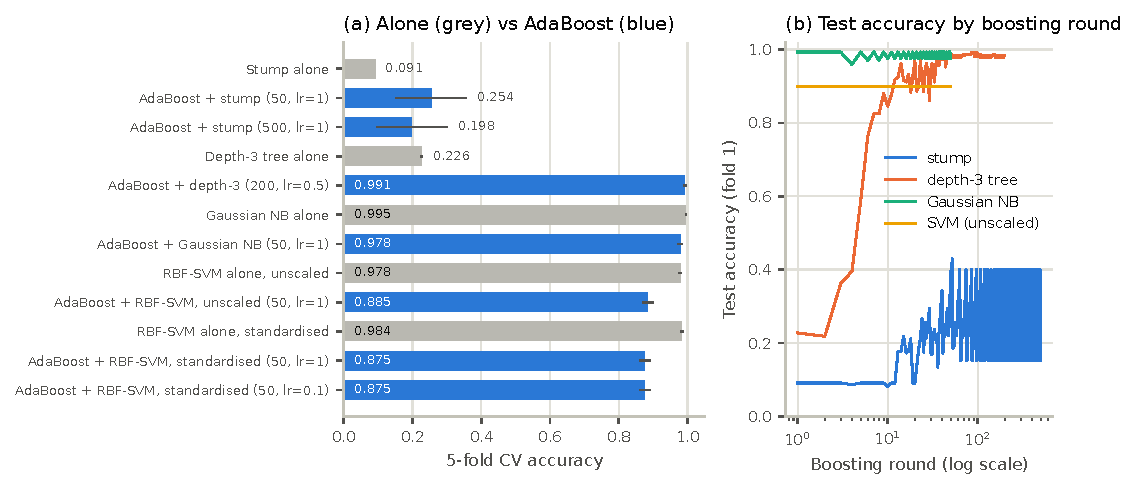
\includegraphics[width=\columnwidth]{figures/fig08_adaboost_diagnosis.pdf}}
\caption{AdaBoost on 22 classes. (a) 5-fold accuracy of each base learner alone (grey) and boosted (blue). (b) Test accuracy by boosting round on one fold.}
\label{fig:ada}
\end{figure}

\subsection{Is 99\% Accuracy Overfitting?}

No. Fig.~\ref{fig:leak}(a) shows train and held-out accuracy for 11 models. The gap is 0.06 percentage points for Gaussian NB, 0.5 for Random Forest and CatBoost, and at most 2.5 for $k$-NN. The tree-depth curve in Fig.~\ref{fig:leak}(b) rises together on train and test and never diverges. With shuffled labels a Random Forest scores 4.6\% on average (maximum 6.1\%; chance is 4.5\%), against 99.6\% with real labels ($p=0.0099$, the smallest value 100 permutations allow).

\begin{figure*}[htbp]
\centerline{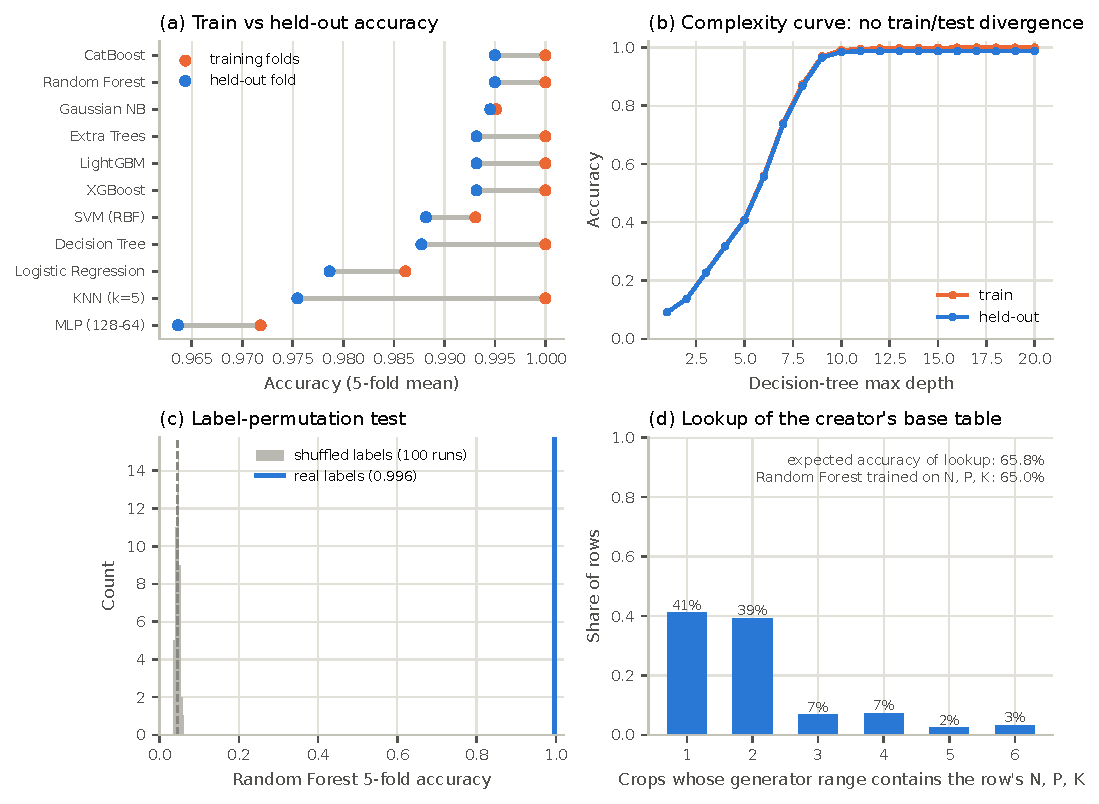
\includegraphics[width=0.82\textwidth]{figures/fig14_overfitting_vs_leakage.pdf}}
\caption{Overfitting versus leakage on the Kaggle crop dataset. (a) Train versus held-out accuracy (5-fold mean). (b) Decision-tree depth curve. (c) Label-permutation test, 100 runs. (d) For each row, the number of crops whose generator box (\ref{eq:gen}) contains its N, P, K; a lookup of the creator's base table reaches 65.8\% expected accuracy, a Random Forest trained on N, P, K reaches 65.0\%.}
\label{fig:leak}
\end{figure*}

The high score has another source. All 2,200 rows satisfy (\ref{eq:gen}), and the observed offsets take exactly 41, 26 and 11 distinct values, the numbers the random ranges allow. A lookup of the base table, with no training, identifies the crop from N, P, K alone with 65.8\% expected accuracy; a Random Forest trained on the same three columns reaches 65.0\% (Fig.~\ref{fig:leak}(d)). The model learns the generator, and the climate columns separate what the N, P, K boxes leave tied. An independent check agrees: of the 154 crop--feature cells, none is consistent with a normal distribution and 82--100\% per feature are consistent with a uniform one.

\subsection{Robustness}

Fig.~\ref{fig:robust} shows that the task is easy for a second reason. With only 8 training rows per crop, a Random Forest reaches 0.974 macro-F1. Small measurement noise, however, hurts the tree models most: at noise of 0.2 standard deviations, LightGBM falls to 0.773, Random Forest to 0.872 and the SVM to 0.947. Feature ablation shows that climate alone (temperature, humidity, rainfall) gives 0.918 macro-F1 for Random Forest while soil alone (N, P, K, pH) gives 0.788; removing rainfall costs the most (0.995 to 0.967).

\begin{figure}[htbp]
\centerline{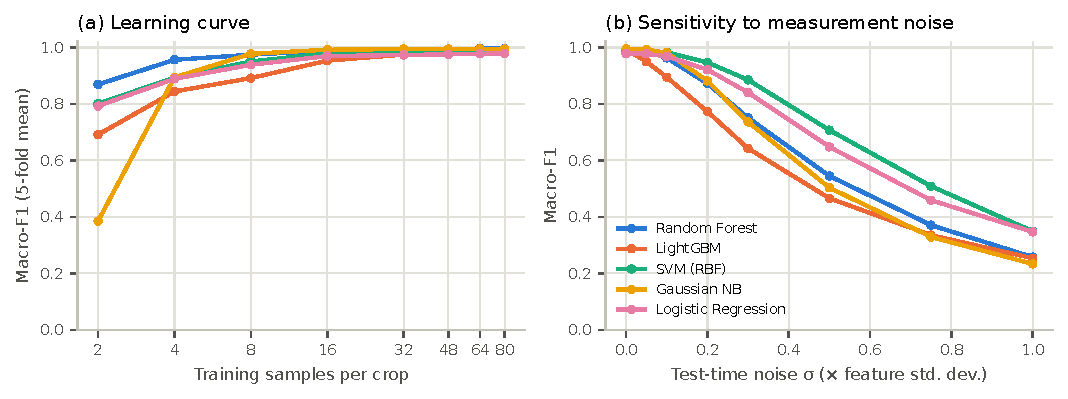
\includegraphics[width=\columnwidth]{figures/fig09_learning_curve_and_noise.pdf}}
\caption{Robustness. (a) Macro-F1 against training rows per crop. (b) Macro-F1 against Gaussian noise added to the test features, in units of each feature's standard deviation.}
\label{fig:robust}
\end{figure}

\subsection{Do the Explanations Agree?}

On random folds the explanations are stable: SHAP rankings across splits have Kendall's $W=0.97$ and all methods name humidity as the top feature in every split. Stability across splits, however, does not show that an explanation is right. Fig.~\ref{fig:xai} tests that more directly.

\begin{figure*}[htbp]
\centerline{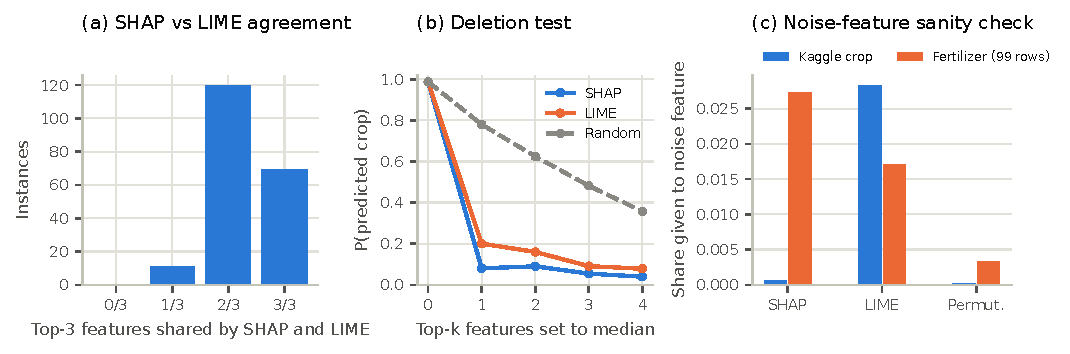
\includegraphics[width=0.85\textwidth]{figures/fig15_xai_disagreement_faithfulness.pdf}}
\caption{Testing the explanations. (a) Top-3 features shared by SHAP and LIME over 200 instances. (b) Deletion test: probability of the predicted crop as the top-$k$ features are set to their median. (c) Share of attribution given to an added pure-noise feature.}
\label{fig:xai}
\end{figure*}

SHAP and LIME share on average 76\% of their top-3 features, name the same top feature in 80\% of instances, and their attribution magnitudes have a Spearman correlation of 0.65; when they share a feature they agree on its sign 98\% of the time. In the deletion test, setting the top SHAP feature to its median drops the probability of the predicted crop from 0.99 to 0.08; the top LIME feature drops it to 0.20 and a random feature to 0.78. On this dataset SHAP is the more faithful of the two. A pure-noise feature is ranked last by all three methods on the crop data.

\textit{Are explanations actionable?} A farmer can change N, P, K and pH but not the climate. With climate fixed, a change in soil alone reaches the target crop for 38\% of instances, and only 40\% of those counterfactuals fall inside the target crop's range in the data; the rest rely on extrapolation (Fig.~\ref{fig:cf}). Most recommended switches cannot be achieved by soil management.

\begin{figure}[htbp]
\centerline{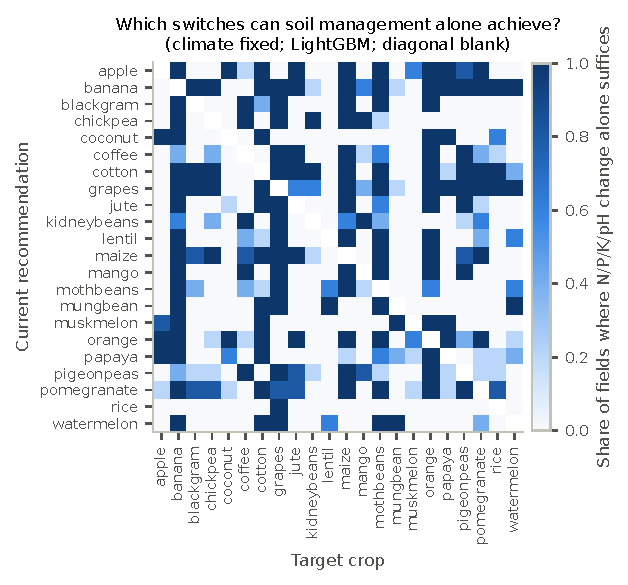
\includegraphics[width=0.85\columnwidth]{figures/fig16_counterfactual_feasibility.pdf}}
\caption{Constrained counterfactuals (LightGBM, climate fixed). Share of instances for which changing only N, P, K and pH moves the recommendation from the current crop (row) to the target crop (column).}
\label{fig:cf}
\end{figure}

\subsection{Calibration and Uncertainty}

High accuracy does not mean reliable probabilities (Fig.~\ref{fig:unc}). Raw ECE is 0.110 for the SVM and 0.040 for Random Forest; isotonic calibration lowers them to 0.007 and 0.004. Split-conformal LAC sets for LightGBM at $\alpha=0.10$ cover the true crop in 89.7\% of cases, matching the target on average, but coverage for the worst crop is only 60.5\%. Average coverage hides crops for which the guarantee fails. APS sets over-cover (99.4\%) at a larger mean set size (1.14).

\begin{figure}[htbp]
\centerline{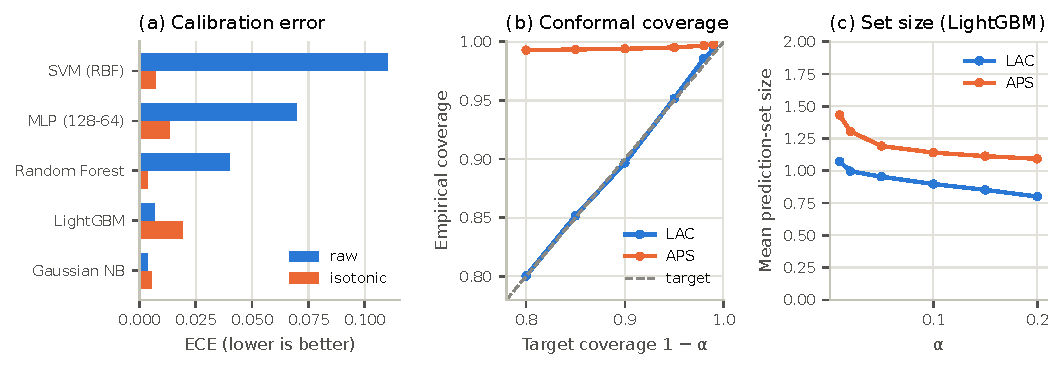
\includegraphics[width=\columnwidth]{figures/fig13_calibration_conformal.pdf}}
\caption{Uncertainty. (a) ECE before and after isotonic calibration. (b) Empirical against target coverage of conformal sets. (c) Mean set size for LightGBM.}
\label{fig:unc}
\end{figure}

\subsection{Comparison of Fertilizer Recommendation}

Table~\ref{tab:fert} compares four models across four feature groups on the 99-row fertilizer dataset. With N, P and K alone, Random Forest, logistic regression and the SVM reach 100\% leave-one-out accuracy. Temperature, humidity and moisture give 16--25\%, and soil type plus crop type give 9--17\%; both are at or below the 22\% majority class. Adding these uninformative features to N, P, K lowers the SVM from 100\% to 67\%.

\begin{table}[htbp]
\caption{Fertilizer Dataset: Leave-One-Out Accuracy (\%) by Feature Group and Model. Majority Class: 22.2\%}
\label{tab:fert}
\centering
\footnotesize
\begin{tabular}{@{}lcccc@{}}
\toprule
\textbf{Features} & \textbf{DT} & \textbf{RF} & \textbf{LR} & \textbf{SVM} \\
\midrule
All features & 97.0 & 96.0 & 85.9 & 66.7 \\
N, P, K only & 97.0 & \textbf{100.0} & \textbf{100.0} & \textbf{100.0} \\
Temp., humidity, moisture & 17.2 & 16.2 & 16.2 & 25.3 \\
Soil type + crop type & 9.1 & 11.1 & 17.2 & 14.1 \\
\bottomrule
\end{tabular}
\end{table}

The reason is in the inputs. Table~\ref{tab:cos} gives the cosine similarity between each class's median N:P:K and the nutrient grade of each fertilizer. For every class the highest similarity is with the grade of its own label (0.991 to 1.000); 20-20 and 28-28 tie because their N:P:K ratios are identical. A decision tree trained on N, P, K reproduces the labels with rules such as ``P $\le$ 4 $\rightarrow$ Urea'' and ``P $>$ 34 $\rightarrow$ DAP'', which restate the composition of the products. Since the construction of the dataset is not documented, we treat this as strong evidence of label mirroring, not proof.

\begin{table}[htbp]
\caption{Cosine Similarity Between Each Class's Median N:P:K (Rows) and the N--P$_2$O$_5$--K$_2$O Grade of Each Fertilizer (Columns). Bold: Row Maximum}
\label{tab:cos}
\centering
\scriptsize
\setlength{\tabcolsep}{3pt}
\begin{tabular}{@{}lccccccc@{}}
\toprule
\textbf{Label} & \textbf{10-26-26} & \textbf{14-35-14} & \textbf{17-17-17} & \textbf{20-20} & \textbf{28-28} & \textbf{DAP} & \textbf{Urea} \\
\midrule
10-26-26 & \textbf{.999} & .909 & .929 & .638 & .638 & .707 & .236 \\
14-35-14 & .888 & \textbf{.991} & .839 & .831 & .831 & .954 & .247 \\
17-17-17 & .951 & .912 & \textbf{.999} & .805 & .805 & .751 & .547 \\
20-20 & .668 & .862 & .816 & \textbf{1.00} & \textbf{1.00} & .916 & .707 \\
28-28 & .646 & .834 & .815 & \textbf{.998} & \textbf{.998} & .886 & .755 \\
DAP & .730 & .936 & .732 & .896 & .896 & \textbf{.999} & .320 \\
Urea & .262 & .348 & .577 & .707 & .707 & .364 & \textbf{1.00} \\
\bottomrule
\end{tabular}
\end{table}

\begin{figure*}[htbp]
\centerline{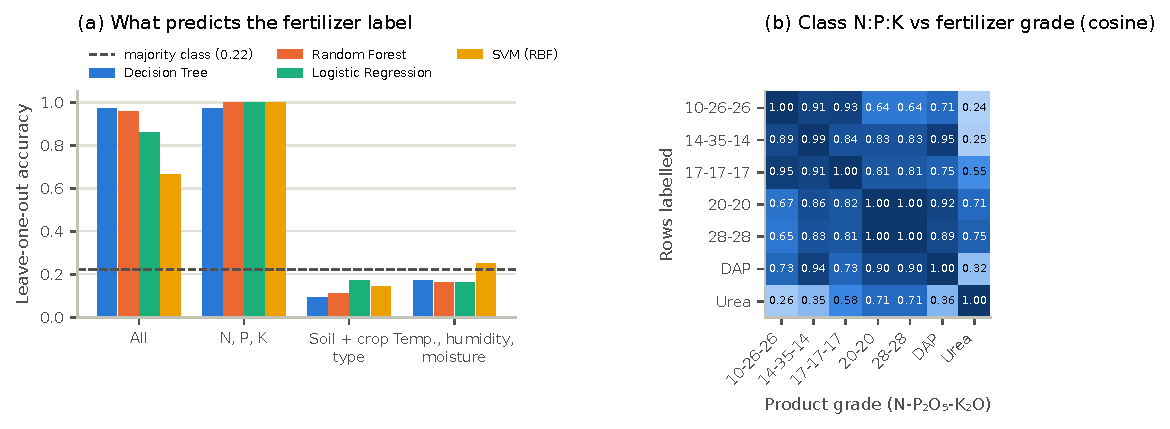
\includegraphics[width=0.85\textwidth]{figures/fig17_fertilizer_benchmark.pdf}}
\caption{Fertilizer benchmark. (a) Leave-one-out accuracy by feature group; dashed line: majority class (0.22). (b) Cosine similarity between each class's median N:P:K and each product's grade.}
\label{fig:fert}
\end{figure*}

The explanations of the fertilizer model mislead in a different way. SHAP assigns 23\% and LIME 36\% of the total attribution to the features that carry no information (temperature, humidity, moisture, soil and crop type), while held-out permutation importance assigns them 2\%. Attribution methods describe what a fitted model uses, not what is predictive.

\textit{A soil-test alternative.} A fertilizer recommendation in practice is a nutrient dose, set from a soil test and a target yield, and then converted into products. Table~\ref{tab:dose} shows the conversion (\ref{eq:dose}) for one published soil-test crop response (STCR) dose for rice of 100--52--25 kg/ha N--P$_2$O$_5$--K$_2$O \cite{icar_iiss}. It also lists the two soil-test rating standards that we plan to compare on real Soil Health Card samples \cite{icar_iiss,tnau_rating}; that comparison is not yet run because the sample-level data are not yet available.

\begin{table}[htbp]
\caption{Dose-to-Product Conversion and Soil-Test Rating Standards}
\label{tab:dose}
\centering
\footnotesize
\begin{tabular}{@{}lccc@{}}
\toprule
\multicolumn{4}{@{}l}{\textbf{(a) STCR rice dose 100--52--25 kg/ha $\rightarrow$ products (kg/ha)}} \\
\midrule
 & \textbf{DAP} (18-46-0) & \textbf{Urea} (46-0-0) & \textbf{MOP} (0-0-60) \\
Quantity & 113.0 & 173.2 & 41.7 \\
\midrule
\multicolumn{4}{@{}l}{\textbf{(b) Low / medium / high thresholds (kg/ha)}} \\
\midrule
\textbf{Standard} & \textbf{N} & \textbf{P} & \textbf{K} \\
ICAR-IISS & $<$280 / -- / $>$560 & $<$10 / -- / $>$25 & $<$120 / -- / $>$280 \\
TNAU & $<$240 / -- / $>$480 & $<$11 / -- / $>$22 & $<$110 / -- / $>$280 \\
\bottomrule
\end{tabular}
\end{table}

\subsection{Discussion}

The two benchmarks show the same pattern. A model scores near 100\% because the inputs were built from, or mirror, the label. On the crop dataset N, P and K are the label plus bounded noise; on the fertilizer dataset N:P:K matches the product's composition. In both cases the remaining features are either copied from an undocumented source or carry no information, and none of this is visible from the accuracy table. A reader of Table~\ref{tab:bench} would conclude that Stacking is the best crop recommender; the significance test says that 11 models are tied, and the provenance check says that none of them has learned agronomy.

The explanations do not raise an alarm either. SHAP correctly reports that humidity, rainfall and N, P, K drive the crop model, because that is what the generator made predictive, and on the fertilizer data it spends almost a quarter of its attribution on features that a held-out test shows are useless. An explanation describes a model; it cannot tell whether the data that shaped the model were real.

\textit{Practical recommendations.} For work on crop or fertilizer recommendation we suggest: (i) check where a dataset came from before reporting accuracy on it; (ii) report significance against the best model and a simple baseline such as Gaussian NB, not only a ranking; (iii) report the train/test gap and a permutation test when claiming that a model does not overfit; (iv) validate explanations with a second method, a deletion test and a noise feature; and (v) report per-class coverage when using conformal sets.

\textit{Threats to validity.} The hyperparameters are fixed, not tuned; tuning could change the order among tied models but not the 99\% ceiling. The fertilizer conclusion rests on a pattern in the data, not on the creator's code, which is not available. All results are on the two public benchmarks; we have not yet shown how the models behave on real field data, which is the main limitation of this paper.

\section{Conclusion and Future Work}

We set out to test what near-perfect accuracy on the two most used crop and fertilizer benchmarks measures. On the crop dataset, 11 of 16 models tie with the best at 98.8--99.6\%, the models do not overfit (gaps at most 2.5 points, permutation $p=0.0099$), and the N, P, K features were generated from the label by a rule that holds for all 2,200 rows; a lookup of that rule alone reaches 65.8\%. On the fertilizer dataset, N, P, K alone give 100\% leave-one-out accuracy, the other features are no better than the majority class, and each class's N:P:K matches its product's grade. SHAP and LIME agree on the top feature in 80\% of instances and assign 23--36\% of the fertilizer model's attribution to useless features. These benchmarks measure recovery of a generating rule, not agronomic skill.

\textit{Future work.} We have built a district-level dataset from government crop statistics (data.gov.in, 34,940 district-season-year rows, 48 crops) on which we will compare random, leave-district-out, leave-state-out and temporal validation, once district soil (Soil Health Card) and climate features are attached. The rating-standard comparison of Table~\ref{tab:dose}(b) will be run on Soil Health Card samples. Results for these experiments are not reported here because they have not been run on real data.

\begin{thebibliography}{00}
\bibitem{kaggle_crop} A. Ingle, ``Crop recommendation dataset,'' Kaggle, 2020. [Online]. Available: \url{https://www.kaggle.com/datasets/atharvaingle/crop-recommendation-dataset}
\bibitem{harvestify} Gladiator07, ``Harvestify,'' GitHub repository, commit aac427c, 2023. [Online]. Available: \url{https://github.com/Gladiator07/Harvestify}
\bibitem{lundberg2017} S. M. Lundberg and S.-I. Lee, ``A unified approach to interpreting model predictions,'' in \textit{Advances in Neural Information Processing Systems}, vol. 30, 2017, pp. 4765--4774.
\bibitem{lundberg2020} S. M. Lundberg \textit{et al.}, ``From local explanations to global understanding with explainable AI for trees,'' \textit{Nature Machine Intelligence}, vol. 2, no. 1, pp. 56--67, 2020.
\bibitem{ribeiro2016} M. T. Ribeiro, S. Singh, and C. Guestrin, ```Why should I trust you?': Explaining the predictions of any classifier,'' in \textit{Proc. 22nd ACM SIGKDD Int. Conf. Knowledge Discovery and Data Mining}, 2016, pp. 1135--1144.
\bibitem{krishna2024} S. Krishna, T. Han, A. Gu, S. Wu, S. Jabbari, and H. Lakkaraju, ``The disagreement problem in explainable machine learning: A practitioner's perspective,'' \textit{Transactions on Machine Learning Research}, 2024.
\bibitem{nadeau2003} C. Nadeau and Y. Bengio, ``Inference for the generalization error,'' \textit{Machine Learning}, vol. 52, no. 3, pp. 239--281, 2003.
\bibitem{bouckaert2004} R. R. Bouckaert and E. Frank, ``Evaluating the replicability of significance tests for comparing learning algorithms,'' in \textit{Advances in Knowledge Discovery and Data Mining (PAKDD)}, LNCS 3056, 2004, pp. 3--12.
\bibitem{holm1979} S. Holm, ``A simple sequentially rejective multiple test procedure,'' \textit{Scandinavian Journal of Statistics}, vol. 6, no. 2, pp. 65--70, 1979.
\bibitem{ojala2010} M. Ojala and G. C. Garriga, ``Permutation tests for studying classifier performance,'' \textit{Journal of Machine Learning Research}, vol. 11, pp. 1833--1863, 2010.
\bibitem{kaufman2012} S. Kaufman, S. Rosset, C. Perlich, and O. Stitelman, ``Leakage in data mining: Formulation, detection, and avoidance,'' \textit{ACM Transactions on Knowledge Discovery from Data}, vol. 6, no. 4, pp. 1--21, 2012.
\bibitem{kapoor2023} S. Kapoor and A. Narayanan, ``Leakage and the reproducibility crisis in machine-learning-based science,'' \textit{Patterns}, vol. 4, no. 9, p. 100804, 2023.
\bibitem{wachter2018} S. Wachter, B. Mittelstadt, and C. Russell, ``Counterfactual explanations without opening the black box: Automated decisions and the GDPR,'' \textit{Harvard Journal of Law \& Technology}, vol. 31, no. 2, pp. 841--887, 2018.
\bibitem{ustun2019} B. Ustun, A. Spangher, and Y. Liu, ``Actionable recourse in linear classification,'' in \textit{Proc. Conf. Fairness, Accountability, and Transparency (FAT*)}, 2019, pp. 10--19.
\bibitem{guo2017} C. Guo, G. Pleiss, Y. Sun, and K. Q. Weinberger, ``On calibration of modern neural networks,'' in \textit{Proc. 34th Int. Conf. Machine Learning (ICML)}, PMLR 70, 2017, pp. 1321--1330.
\bibitem{sadinle2019} M. Sadinle, J. Lei, and L. Wasserman, ``Least ambiguous set-valued classifiers with bounded error levels,'' \textit{Journal of the American Statistical Association}, vol. 114, no. 525, pp. 223--234, 2019.
\bibitem{romano2020} Y. Romano, M. Sesia, and E. J. Cand\`es, ``Classification with valid and adaptive coverage,'' in \textit{Advances in Neural Information Processing Systems}, vol. 33, 2020, pp. 3581--3591.
\bibitem{angelopoulos2021} A. N. Angelopoulos and S. Bates, ``A gentle introduction to conformal prediction and distribution-free uncertainty quantification,'' arXiv:2107.07511, 2021.
\bibitem{breiman2001} L. Breiman, ``Random forests,'' \textit{Machine Learning}, vol. 45, no. 1, pp. 5--32, 2001.
\bibitem{freund1997} Y. Freund and R. E. Schapire, ``A decision-theoretic generalization of on-line learning and an application to boosting,'' \textit{Journal of Computer and System Sciences}, vol. 55, no. 1, pp. 119--139, 1997.
\bibitem{zhu2009} J. Zhu, H. Zou, S. Rosset, and T. Hastie, ``Multi-class AdaBoost,'' \textit{Statistics and Its Interface}, vol. 2, no. 3, pp. 349--360, 2009.
\bibitem{chen2016} T. Chen and C. Guestrin, ``XGBoost: A scalable tree boosting system,'' in \textit{Proc. 22nd ACM SIGKDD Int. Conf. Knowledge Discovery and Data Mining}, 2016, pp. 785--794.
\bibitem{ke2017} G. Ke \textit{et al.}, ``LightGBM: A highly efficient gradient boosting decision tree,'' in \textit{Advances in Neural Information Processing Systems}, vol. 30, 2017, pp. 3146--3154.
\bibitem{prokhorenkova2018} L. Prokhorenkova, G. Gusev, A. Vorobev, A. V. Dorogush, and A. Gulin, ``CatBoost: Unbiased boosting with categorical features,'' in \textit{Advances in Neural Information Processing Systems}, vol. 31, 2018.
\bibitem{wolpert1992} D. H. Wolpert, ``Stacked generalization,'' \textit{Neural Networks}, vol. 5, no. 2, pp. 241--259, 1992.
\bibitem{pedregosa2011} F. Pedregosa \textit{et al.}, ``Scikit-learn: Machine learning in Python,'' \textit{Journal of Machine Learning Research}, vol. 12, pp. 2825--2830, 2011.
\bibitem{grinsztajn2022} L. Grinsztajn, E. Oyallon, and G. Varoquaux, ``Why do tree-based models still outperform deep learning on typical tabular data?'' in \textit{Advances in Neural Information Processing Systems}, vol. 35 (Datasets and Benchmarks Track), 2022.
\bibitem{roberts2017} D. R. Roberts \textit{et al.}, ``Cross-validation strategies for data with temporal, spatial, hierarchical, or phylogenetic structure,'' \textit{Ecography}, vol. 40, no. 8, pp. 913--929, 2017.
\bibitem{icar_iiss} ICAR--Indian Institute of Soil Science, \textit{Harit Dhara}, vol. 4, no. 1, 2021. % TODO: add article title, authors and pages after opening the source.
\bibitem{tnau_rating} TNAU Agritech Portal, ``Soil fertility rating chart,'' Tamil Nadu Agricultural University. [Online]. Available: \url{https://agritech.tnau.ac.in} % TODO: exact page URL and access date.
\end{thebibliography}

\end{document}
